\documentclass[unicode,9pt, pdf]{beamer}
\usepackage{amsmath}
\usepackage[T2A]{fontenc}
\usepackage[utf8]{inputenc}
\usepackage[english, russian]{babel}
\usepackage{amsthm}
\usepackage{booktabs}
\usepackage{graphicx}
\usepackage{caption}
\usepackage{xcolor}
\usepackage{algorithm,algorithmic}

\renewcommand{\algorithmicrequire}{\textbf{Input:}}
\renewcommand{\algorithmicensure}{\textbf{Output:}}
% Table float box with bottom caption, box width adjusted to content
\DeclareGraphicsExtensions{.png}
\graphicspath{{images/}}  
\usetheme{Warsaw}
\usetheme[numbers, minimal,totalnumbers,nonav]{Statmod}
\subject{Beamer}




\title{Тематическое моделирование}

\author[Зенкова Н., Калина Е., Балагуров В.]{Зенкова Наталья \\
        Калина Екатерина \\
        Балагуров Владимир}
\institute[СПбГУ]{Санкт-Петербургский государственный университет \\
	Прикладная математика и информатика \\
	Статистическое моделирование\\

}
\date{
	Санкт-Петербург\\
	2019г.
}


\begin{document}
	
	\begin{frame}
		\titlepage
	\end{frame}
	
	\begin{frame}{Введение}
	
	\textbf{Дано:} Несколько миллионов документов.
	
	\vspace{0.4 cm}
	
	\textbf{Задача:}
	Выявить тематики в текстовой коллекции (какие темы существуют в наших документах?).
	
	\vspace{0.4 cm}
	
	\textcolor{red}{Что такое <<тема>>?}
	
	\vspace{0.4 cm}
	
	\begin{itemize}
	    \item Тема --- специальная терминология предметной области;
	    \vspace{0.2 cm}
	    \item Тема --- набор часто совместно встречающихся терминов;
	    \vspace{0.2 cm}
	    \item Тема --- семантически однородный кластер текстов.
	\end{itemize}
	
	


	\end{frame}
	   \begin{frame}{Некоторые приложения тематического моделирования}
        \begin{itemize}
            \item Разведочный поиск в электронных библиотеках;
            \vspace{0.3 cm}
            \item Поиск тематического контента в соцсетях;
            \vspace{0.3 cm}
            \item Детектирование и трекинг новостных сюжетов;
            \vspace{0.3 cm}
            \item Мультимодальный поиск текстов и изображений;
            \vspace{0.3 cm}
            \item Анализ банковских транзакционных данных.
        \end{itemize}
    \end{frame}

 \begin{frame}{Пусть}
    
    \begin{itemize}
        \item $D$ --- конечное множество (коллекция) текстовых документов;
        \item $W$ --- конечное множество слов (терминов, токенов);
        \item $T$ --- конечное множество тем;
         \item $D \times W \times T$ --- дискретное вероятностное простанство;
         \item Коллекция --- это i.i.d выборка $(d_i, w_i, t_i)^n_{i=1} \sim p(d, w, t)$.
     \end{itemize}
     
     \vspace{0.2 cm}
     
     Каждый документ $d \in D$ представляет собой последовательность $n_d$ терминов $(w_1, \ldots, w_{n_d})$ из словаря $W$. Термин может повторяться в документе много раз.
     
     \vspace{0.2 cm}
     
     \textcolor{red}{$d_i$, $w_i$ --- наблюдаемые величины, $t_i$ --- скрытые}
     
     \vspace{0.2 cm}
     
     \textbf{Задача тематического моделирования:} Найти множество тем $T$, распределение $p(w|t)$ для всех тем $t \in T$, распределение $p(t|d)$ для всех документов.
     
     \vspace{0.3 cm}
     
     
     Далее, найденные распределения могут использоваться для решения прикладных задач.
     
     \end{frame}
	

    \begin{frame}{Что такое <<тема>> в коллекции текстовых документов?}
    
     \begin{itemize}
         \item 
         \textcolor{blue}{$p(w|t)$} --- вероятность термина $w$ в теме $t$;
         \vspace{0.4 cm}
         \item  \textcolor{blue}{$p(t|d)$} --- вероятность темы $t$ в документе $d$.
     \end{itemize}
     
     \vspace{0.4 cm}
     
    Когда автор писал термин $w$ в документе $d$, он думал о теме $t$, и мы хотели бы выявить, о какой именно.
    
    \vspace{0.4 cm}
    \textit{Тематическая модель} выявляет латентные (скрытые) темы по наблюдаемым распределениям слов $p(w|d)$ в документах.
     
     \vspace{0.4 cm}
     
     \textbf{Отличие от кластеризации:}
     \begin{itemize}
         \item \textcolor{blue}{Жесткая кластеризация:} кластеризация текстов новостей (относим новостное событие к определенной теме);
         \item \textcolor{blue}{Мягкая кластеризация:} кластеризация научных статей (много исследований находятся на стыке наук).
     \end{itemize}
     Документ $d$ может быть связан с \textcolor{red}{несколькими} темами $t$.
    \end{frame}
    
 
   
     
     \begin{frame}{Гипотезы и предположения}
     
     \textbf{Гипотеза независимости:} Порядок слов в документе и порядок документов в коллекции не важны.
     
     \vspace{0.4 cm}
     
     \textbf{Гипотеза условной независимости:} $p(w|d,t) = p(w|t)$.
     
     \vspace{0.4 cm}
     
     \textbf{Гипотеза разреженности:} Каждый документ $d$ и каждый термин $w$ связан с небольшим количеством тем $t$. 
     
      \vspace{0.2 cm}
      
     \textcolor{red}{Как получить разреженность?}
     \vspace{0.2 cm}
     
      \begin{itemize}
          \item Документ относится к большому количеству тем.\\
           \vspace{0.2 cm}
           \textit{Решение:} разобьем его на части, более однородные по тематике.
           \vspace{0.2 cm}
          \item Термин относится к большому числу тем.\\
            \vspace{0.2 cm}
            \textit{Решение:} положим, что термин является общеупотребительным словом и несет мало полезной информации с точки зрения тематики.

      \end{itemize}
     
      \vspace{0.4 cm}
      
     \textbf{Тематическая модель} по формуле полной вероятности:
     \begin{gather*}
        p(w|d) = \sum_{t \in T}p(w|t)p(t|d).
     \end{gather*}
    
    \end{frame}
 
     
   \begin{frame}{Предварительная обработка документов}
   \textbf{Мотивация:} Для упрощения модели прибегают к предварительной обработке текстов.
   
   \begin{itemize}
       \item \textit{Лемматизация} --- приведение каждого слова в документе к его нормальной форме.\\
       \vspace{0.1 cm}
       \textcolor{blue}{Трудоемкий процесс}
       \vspace{0.1 cm}  
       \item \textit{Стемминг} --- отбрасывание изменяемых частей слова.\\
    \vspace{0.1 cm}
       \textcolor{blue}{Большое число ошибок}
       \vspace{0.1 cm}      
       \item \textit{Уменьшение словаря:}\\
       \vspace{0.1 cm}
       \begin{itemize}
           \item $1000, 5, 23 \to \text{\$number}$,
           \vspace{0.2 cm}
           $(5+3)$, $\frac{1}{2}\mathbf{w}\mathbf{w}^{\mathrm{T}} + C \to \text{\$formula}$.
           \vspace{0.1 cm} 
           \item \textit{Отбрасывание стоп-слов} --- удаление слов (предлогов, союзов, вводных слов и т.д.), которые никак не характеризуют тему.\\
           \textcolor{blue}{Почти не влияет на длину словаря}
            \vspace{0.1 cm} 
           \item \textit{Отбрасывание редких слов.}\\
          \textcolor{blue}{Для коллекций коротких новостных сообщений лучше не использовать}
           \vspace{0.1 cm} 
           \item \textit{Выделение ключевых фраз.}\\
             \textcolor{blue}{Приходится привлекать экспертов}
       \end{itemize} 
   \end{itemize}

   \end{frame}
   
   \begin{frame}{Прямая задача --- порождение коллекиции по $p(w|t)$ и $p(t|d)$}
   \textit{Тематическая модель} по формуле полной вероятности:
   \begin{gather*}
       p(w|d) = \sum_{t \in T} p(w|d,t)p(t|d) = \sum_{t \in T} p(w|t) p(t|d), \text{ где}
   \end{gather*}
\begin{itemize}
    \item $p(w|t)$ --- распределение терминов в каждой теме,
    \item $p(t|d)$ --- распределение тем в каждом документе.
\end{itemize}
   	\begin{center}
		\centering
		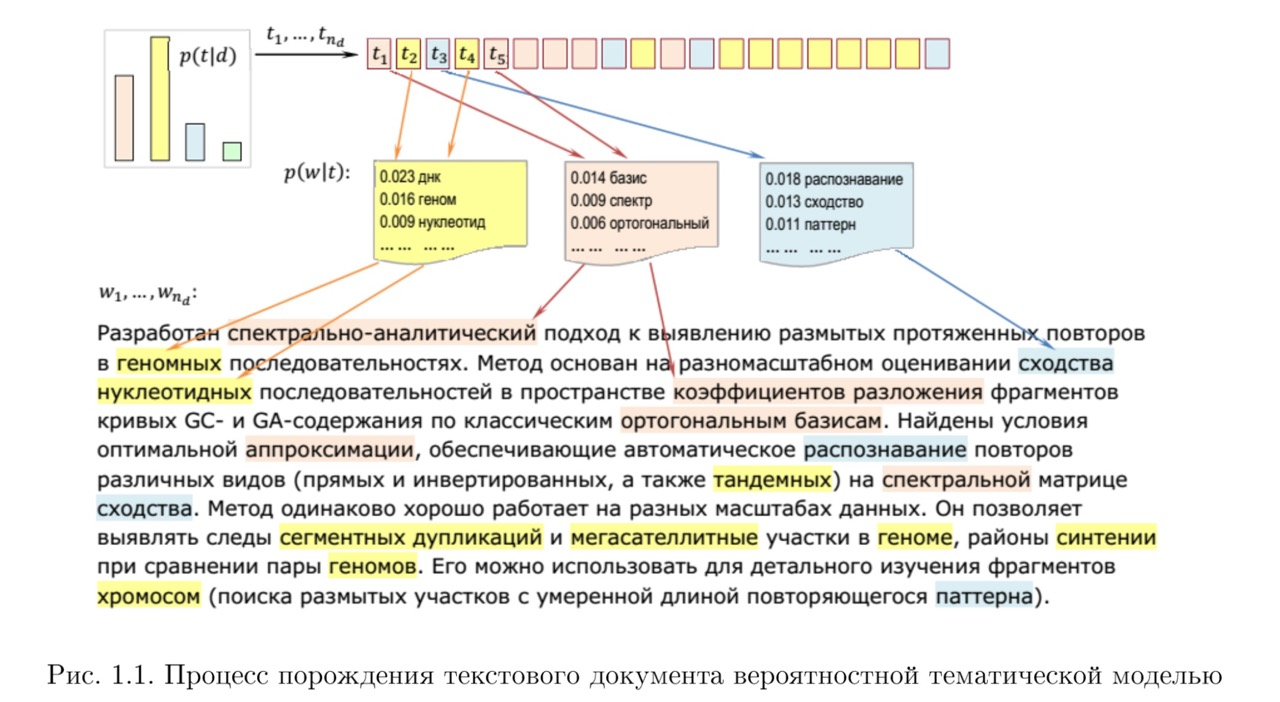
\includegraphics[width=230pt, height=120pt]{Picture1.jpg}
	\end{center}
   
   \end{frame}
   
   \begin{frame}{Обратная задача --- восстановление $p(w|t)$ и $p(t|d)$ по коллекции}
   
   \textbf{Дано:} коллекция текстовых документов
       \begin{itemize}
           \item $n_{d w}$ --- частоты терминов в документах, $\hat{p}(w|d) = \frac{n_{d w}}{n_{d}}$
       \end{itemize}
      
      \textbf{Найти:} параметры тематической модели $p(w|d) = \sum_{t \in T} \phi_{w t} \theta_{t d}$
      \begin{itemize}
          \item $\phi_{w t} = p(w|t)$ --- вероятности терминов $w$ в каждой теме $t$
          \item $\theta_{t d} = p(t|d)$ --- вероятности тем $t$ в каждом документе $d$
      \end{itemize}
      
      Это задача стохастического матричного разложения:
      \begin{center}
		\centering
		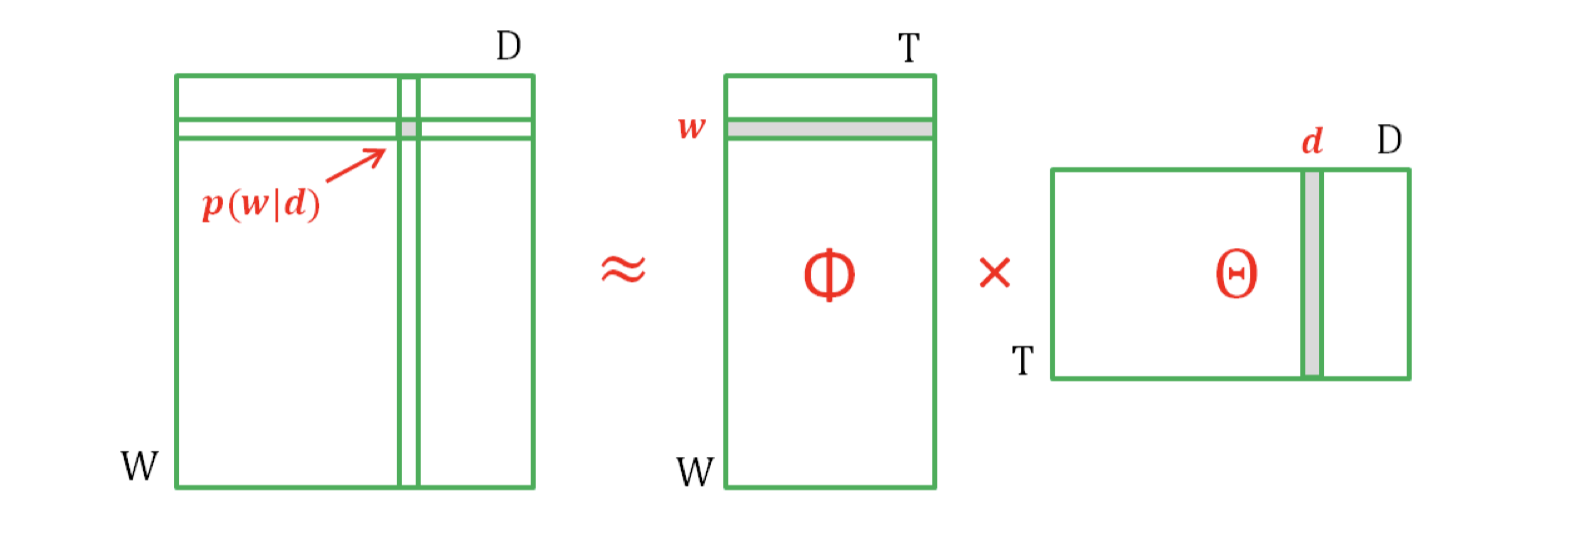
\includegraphics[width=270pt, height=100pt]{Picture2.png}
	\end{center}
	
	\begin{itemize}
	   % \item Столбцы матриц неотрицательны и нормированы.
	    \item Если $\mathbf{\Phi}$ и $\mathbf{\Theta}$ --- решение, то
	    существует матрица $\mathbf{S}$ ранга $|T|$ такая, что $\mathbf{\Phi}^{'}\mathbf{\Theta}^{'} = (\mathbf{\Phi} \mathbf{S})(\mathbf{S}^{-1}\mathbf{\Theta})$, но $\mathbf{\Phi}^{'}$ и $\mathbf{\Theta}^{'}$ \textcolor{red}{не обязательно стохастические.}
	\end{itemize}
	
	

      


   \end{frame}
   
   \begin{frame}{Оценки вероятностей}
   \textbf{Наблюдаемые частоты:}
   $$\hat{p}(d, w) = \frac{n_{d w}}{n}, \hspace{0.2 cm} \hat{p}(d) = \frac{n_d}{n}, \hspace{0.2 cm} \hat{p}(w) = \frac{n_{w}}{n}, \hspace{0.2 cm} \hat{p}(w, d) = \frac{n_{d w}}{n_d}, \text{ где}$$
   \begin{itemize}
       \item $n_{d w}$ --- число вхождений термина $w$ в документ $d$;
       \item $n_d = \sum_{w \in W} n_{d w}$ --- длина документа $d$ в терминах;
       \item $n_w = \sum_{d \in D}n_{d w}$ --- число вхождений термина $w$ во все документы коллекции;
       \item $n = \sum_{d \in D} \sum_{w \in W} n_{d w}$ --- длина коллекции $d$ в терминах.
       \end{itemize}
       
       \vspace{0.2 cm}
       
       \textbf{Ненаблюдаемые частоты, связанные с $t$}:
       
       $$\hat{p}(t) = \frac{n_t}{n}, \hspace{0.2 cm} \hat{p}(w|t) = \frac{n_{w t}}{n_t}  \hspace{0.2 cm} \hat{p}(t|d) = \frac{n_{d t}}{n_d} \hspace{0.2 cm} \hat{p}(t|d, w) = \frac{n_{d w t}}{n_{d w}} \text{ где}$$
   \begin{itemize}
       \item $n_{d w t}$ --- число троек, в которых термин $w$ в документе $d$ связан с темой $t$;
       \item $n_{d t} = \sum_{w \in W} n_{d w t}$ --- число троек, в которых термин в документе $d$ связан с темой $t$;
       \item $n_{w t} = \sum_{d \in D} n_{d w t}$ --- число троек, в которых термин $w$ связан с темой~$t$;
       \item $n_t = \sum_{d \in D} \sum_{w \in W} n_{d w t}$ --- число троек, связанных с темой $t$.
   \end{itemize}
       
   \end{frame}
   
   \begin{frame}{Вероятностный латентный семантический анализ (PLSA)}
   Рассмотрим один из способов описания тематической модели представления коллекции текстовых документов.
   \begin{gather*}
      \mathbf{F} \approx \mathbf{\Phi}\mathbf{\Theta}, \text{ где } \mathbf{\Phi} = (\phi)_{W \times T}, \phi_{w t} = p(w|t); \hspace{0.2 cm} \mathbf{\Theta} = (\theta)_{T \times D}, \theta_{t d} = p(t|d).
   \end{gather*}
   
   Для оценивания параметров $\mathbf{\Phi}$ и $\mathbf{\Theta}$ тематической модели будем максимизировать функцию правдоподобия:
   \begin{gather*}
       \mathcal{L}(\mathbf{\Phi}, \mathbf{\Theta}) = C \prod_{d \in D} \prod_{w \in d} p(d, w)^{n_{d w}} = \prod_{d \in D} \prod_{w \in d} p(w|d)^{n_{d w}} \underbrace{C p(d)^{n_{d w}}}_{const} \to \max_{\mathbf{\Phi}\mathbf{\Theta}},
   \end{gather*}
   где $C$ --- нормировочный множитель.
      
      \vspace{0.2 cm}
      
      \textbf{Задача максимума правдоподобия с ограничениями:}
       
     \begin{gather*}
        \begin{cases}
        \mathcal{L}_{\log}(\mathbf{\Phi}, \mathbf{\Theta}) = \prod\limits_{d \in D} \prod\limits_{w \in d} n_{d w} \ln{\sum\limits_{t \in T} \phi_{w t} \theta_{t d}} \to \max\limits_{\mathbf{\Phi}\mathbf{\Theta}}\\
        \phi_{w t} \geq 0, \sum\limits_{w \in W} \phi_{w t} = 1\\
        \theta_{t d} \geq 0, \sum\limits_{t \in T}\theta_{t d} = 1.
        \end{cases}
     \end{gather*}
      \textcolor{red}{Для решения задачи применяется ЕМ-алгоритм}
   \end{frame}
   
   \begin{frame}{PLSA: ЕМ-алгоритм}
   \textbf{Е-шаг.} Вычисляются условные вероятности $p(t|d, w)$ всех тем $t \in T$ для каждого термина $w \in W$ в каждом документе $d$:
   \begin{gather*}
       H_{d w t} = p(t|d, w) = \frac{p(w|t) p(t|d)}{p(w|d)} = \frac{\phi_{w t} \theta_{t d}}{\sum_{s \in T} \phi_{w s} \theta_{s d}}.
   \end{gather*}
   
   \textbf{М-шаг.} По условным вероятностям тем $H_{d w t}$ вычисляется новое приближение параметров $\phi_{w t}$ и $\theta_{t d}$:
 \begin{gather*}
    \phi_{w t} = \frac{\hat{n}_{w t}}{\hat{n}_t}, \hspace{0.2 cm} \hat{n}_{w t} = \sum_{d \in D}n_{d w} H_{d w t}, \hspace{0.2 cm}  \hat{n}_t = \sum_{w \in W}\hat{n}_{w t};\\
    \theta_{t d} = \frac{\hat{n}_{d t}}{\hat{n}_d}, \hspace{0.2 cm}  \hat{n}_{d t} = \sum_{w \in d} n_{d w} H_{d w t}, \hspace{0.2 cm}  \hat{n}_d = \sum_{t \in T} \hat{n}_{d t}.
\end{gather*}



       
   \end{frame}
   
\begin{frame}{Начальное приближение $\phi_{w t}$ и $\theta_{t d}$}
\begin{enumerate}
    \item Начальное приближение можно задать нормированными случайными векторами из равномерного распределения. 
    \item Пройти по всей коллекции, выбрать для каждой пары $(d, w)$ случайную тему $t$, вычислить частотные оценки вероятностей $\phi_{w t}$ и $\theta_{t d}$ для всех $d$, $w$, $t$.
\end{enumerate}

\textbf{Частичное обучение} (некоторые $t$ известны заранее и имеются дополнительные данные о привязке некоторых $d$ или $w$ к $t$):
    \begin{itemize}
        \item Известно, что документ $d$ относится к подмножеству $T_d \subset T$:
        \begin{gather*}
            \theta_{t d}^0 = \frac{1}{W_t} \mathbb{I}_{t \in T_d}.
        \end{gather*}
        \item Известно, что подмножество терминов $W_t \subset W$ относится к теме $t$:
        \begin{gather*}
            \phi_{t d}^0 = \frac{1}{W_t} \mathbb{I}_{w \in W_t}.
        \end{gather*}
        \item Известно, что некоторое множество документов $D_t \subset D$ относится к теме $t$:
        \begin{gather*}
        \phi_{t d}^0 = \frac{\sum_{d \in D} n_{d w}}{\sum_{d \in D_t} n_d}.
        \end{gather*}
    \end{itemize}
\end{frame}

\begin{frame}{Недостатки PLSA}
\begin{enumerate}
    \item Медленно сходится на больших коллекциях, так как $\mathbf{\Phi}$ и $\mathbf{\Theta}$ обновляются после каждого прохода коллекции.
    
    \hspace{0.1 cm}
    
    \item Не разреживает распределение $H_{d w t} = p(t| d, w)$.
    
    \hspace{0.1 cm}
    
    \item Вынуждены хранить матрицу $\mathbf{H} = (H_{d w t})_{D \times W \times T}$.
    
    \hspace{0.1 cm}
    
    \item Слишком много параметров $\phi_{w t}$ и $\theta_{t d}$ ($|W||T| + |T||D|)$.
    
    \hspace{0.1 cm}
    
    \item Неверно оценивает вероятность новых слов ($\hat{p}(w|t) = 0$ для слова, которого не было в обучающейся коллекции, но оно встретилось в каком-нибудь документе).
    
    \hspace{0.1 cm}
    
    \item Не позволяет управлять разреженностью $\mathbf{\Phi}$ и $\mathbf{\Theta}$:
    \begin{gather*}
        (\text{в начале } \phi_{w t} = 0) \Leftrightarrow  (\text{в конце }  \phi_{w t} = 0),\\
         (\text{в начале }  \theta_{t d} = 0) \Leftrightarrow  (\text{в конце } \theta_{t d} = 0).
    \end{gather*}
\end{enumerate}
    
\end{frame}

\begin{frame}{Модификация}
\textbf{Проблема:} Вынуждены хранить матрицу $\mathbf{H} = (H_{d w t})_{D \times W \times T}$.\\

\vspace{0.2 cm}

\textbf{Решение:} Вычислять $H_{d w t}$ по мере необходимости.

\begin{algorithm}[H]
\begin{algorithmic}[1]
\REQUIRE Коллекция $D$, число тем $T$, начальные $\mathbf{\Phi}$ и $\mathbf{\Theta}$
\ENSURE Распределения $\mathbf{\Phi}$ и $\mathbf{\Theta}$
\REPEAT
\STATE обнулить $\hat{n}_{w t}, \hat{n}_{d t}, \hat{n}_t$ для всех $d \in D$, $w \in W$, $t \in T$;
\FORALL{$d \in D$, $w \in d$}
\STATE $Z:=\sum_{t \in T} \phi_{w t} \theta_{t d}$;
\FORALL{$t \in T$ таких, что $\phi_{w t} \theta_{t d} > 0$}
\STATE увеличить $\hat{n}_{w t}, \hat{n}_{d t}, \hat{n}_t$ на $\frac{n_{d w}}{Z}\phi_{w t} \theta_{t d}$;
\ENDFOR
\ENDFOR\\

$\phi_{w t} := \hat{n}_{w t}/\hat{n}_t$ для всех $w \in W$, $t \in T$;\\
$\theta_{t d} := \hat{n}_{d t}/n_d$ для всех $d \in D$, $t \in T$;
\UNTIL{$\mathbf{\Phi}$ и $\mathbf{\Theta}$ не стабилизируются;}
\end{algorithmic}
\caption{Рациональный ЕМ-алгоритм}
\label{alg:seq}
\end{algorithm}
\end{frame}

\begin{frame}{Модификация}
\textbf{Проблема:}{PLSA медленно сходится на больших коллекциях.}

\vspace{0.2 cm}

\textbf{Решение:} Обновлять значения $\mathbf{\Phi}$ и $\mathbf{\Theta}$ чаще.
\begin{algorithm}[H]
\begin{algorithmic}[1]
\REQUIRE Коллекция $D$, число тем $T$, начальные $\mathbf{\Phi}$ и $\mathbf{\Theta}$
\ENSURE Распределения $\mathbf{\Phi}$ и $\mathbf{\Theta}$\\
\STATE Обнулить $\hat{n}_{w t}, \hat{n}_{d t}, \hat{n}_t$, $\hat{n}_d$, $\hat{n}_{d w t}$ для всех $d \in D$, $w \in W$, $t \in T$;
\REPEAT
\FORALL{$d \in D$, $w \in d$}
\STATE $Z:=\sum_{t \in T} \phi_{w t} \theta_{t d}$;
\FORALL{$t \in T$ таких, что $n_{d w t} > 0$ или $\phi_{w t} \theta_{t d} > 0$}
\STATE увеличить $\hat{n}_{w t}$, $\hat{n}_{d t}$, $\hat{n}_t$, $\hat{n}_d$ на $\frac{n_{d w}}{Z}\phi_{w t} \theta_{t d} - n_{d w t}$;\\
$n_{d w t} := \frac{n_{d w}}{Z} \phi_{w t} \theta_{t d} - n_{d w t}$;
\ENDFOR
\IF{не первая итерация и пора обновить параметры $\mathbf{\Phi}$ и $\mathbf{\Theta}$}
\STATE $\phi_{w t} := \hat{n}_{w t}/\hat{n}_t$ для всех $w \in W$, $t \in T$ таких, что $\hat{n}_{w t}$ изменился;\\

$\theta_{t d} := \hat{n_{d t}}/\hat{n}_d$ для всех $d \in D$, $t\in T$ таких, что $\hat{n}_{t d}$ изменился;
\ENDIF
\ENDFOR
\UNTIL{$\mathbf{\Phi}$ и $\mathbf{\Theta}$ не стабилизируются;}
\end{algorithmic}
\caption{Обобщенный ЕМ-алгоритм}
\label{alg:seq}
\end{algorithm}
    
\end{frame}

\begin{frame}{Модификация обобщенного ЕМ-алгоритма}
\textbf{Проблема:} Необходимо хранить массив $n_{d w t} = n_{d w} H_{ d w t}$, который занимает $O(n|T|)$ памяти.\\

\hspace{0.4 cm}

\textbf{Решение:} На М-шаге вместо распределения $H_{d w t} \equiv p(t|d, w)$ взять его несмещенную эмпирическую оценку:

\begin{gather*}
\hat{H}_{d w t} = \hat{p}(t| d, w) = \frac{1}{s}\sum\limits_{i=1}^s \mathbb{I}_{t_{d w i} = t}.
\end{gather*}

В ряде публикаций предложено экономное сэмплирование, когда $s$ уменьшается до 3–5 тем,что приводит к большему разреживанию и экономии вычислительных ресурсов без существенной потери качества тематической модели.
\end{frame}
  
       

\end{document}

